\chapter{Apêndice}\label{chapter:apendice}

% -----------------------------------------------------------------------------
% Capítulo A.1 - Criação de uma política IAM
% -----------------------------------------------------------------------------
\section{Criação de uma política para o AWS IoT}\label{section:criacao_de_uma_politica_para_o_aws_iot}

A sequência de figuras apresentam capturas de telas do processo de criação de uma política para o AWS IoT.

Acesse a \href{https://us-east-1.console.aws.amazon.com/iot/home?region=us-east-1#/home}{página principal do serviço AWS IoT}, expanda a opção \textit{Segurança} e selecione \textit{Políticas}.

\begin{figure}[H]
    \centering
    \caption{Criando uma política no AWS IoT (A).}
    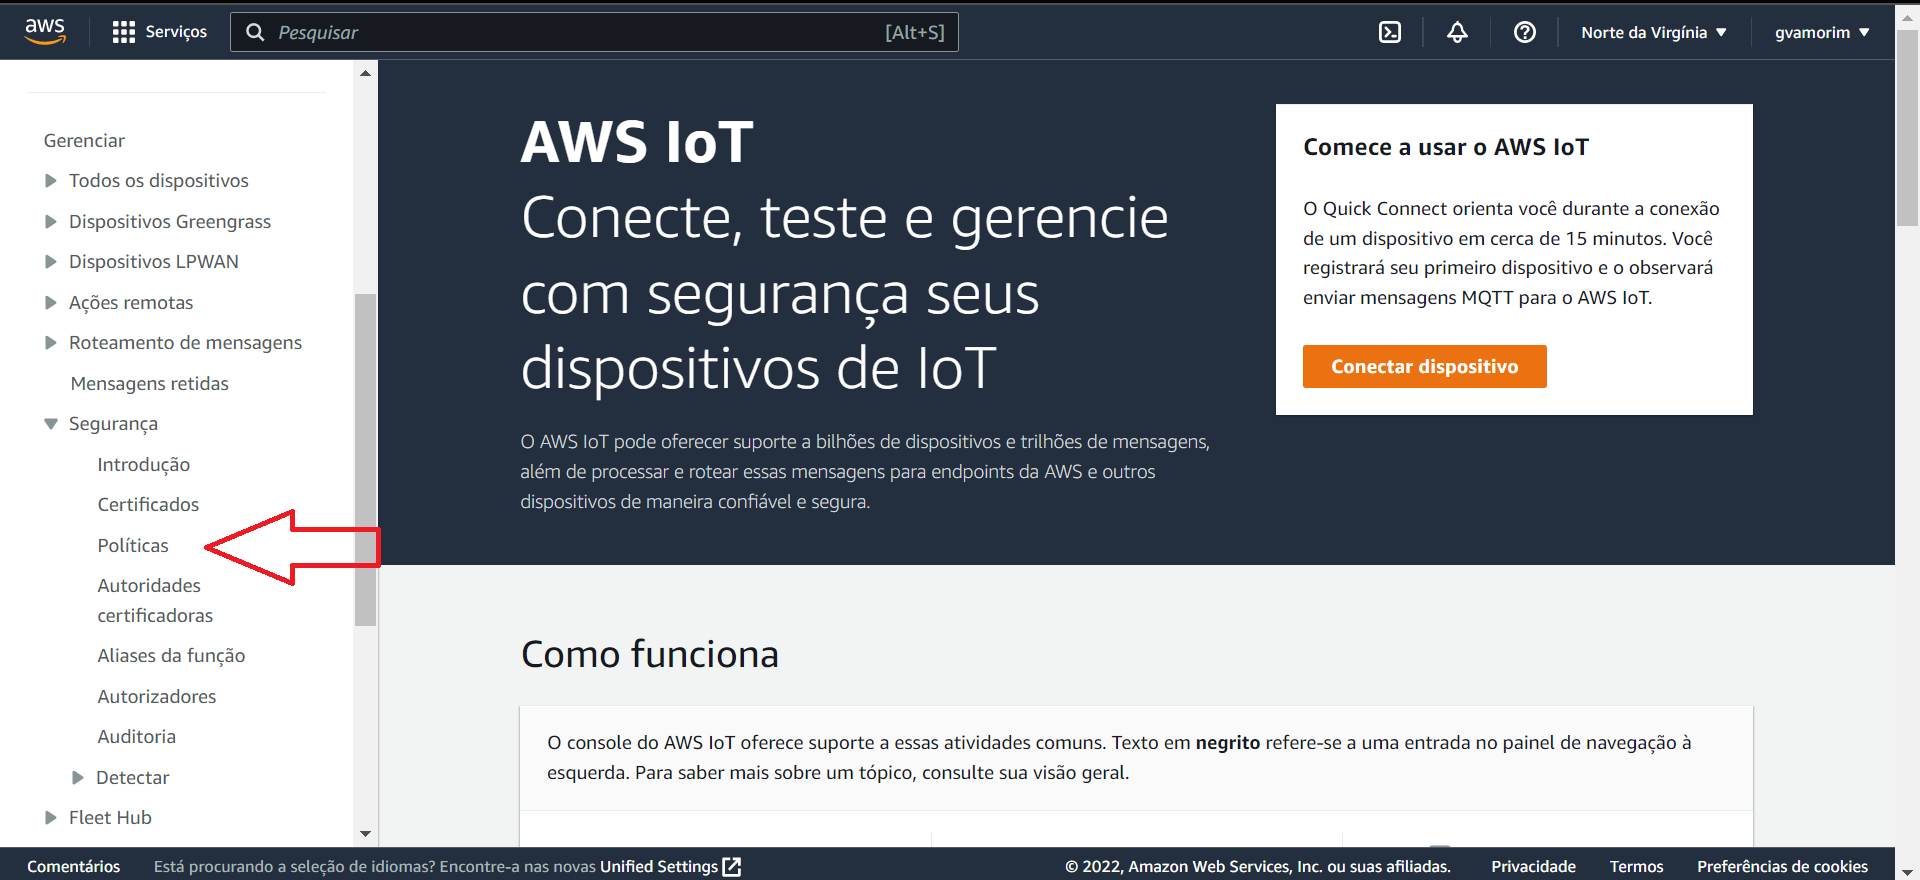
\includegraphics[scale=0.472]{Imagens/criando_uma_politica_no_aws_iot_0.png}
    \legend{Fonte: Produzido pelo autor (2022).}
    \label{fig:criando_uma_politica_no_aws_iot_a}
\end{figure}

Selecione a opção \textit{Criar política}.

\begin{figure}[H]
    \centering
    \caption{Criando uma política no AWS IoT (B).}
    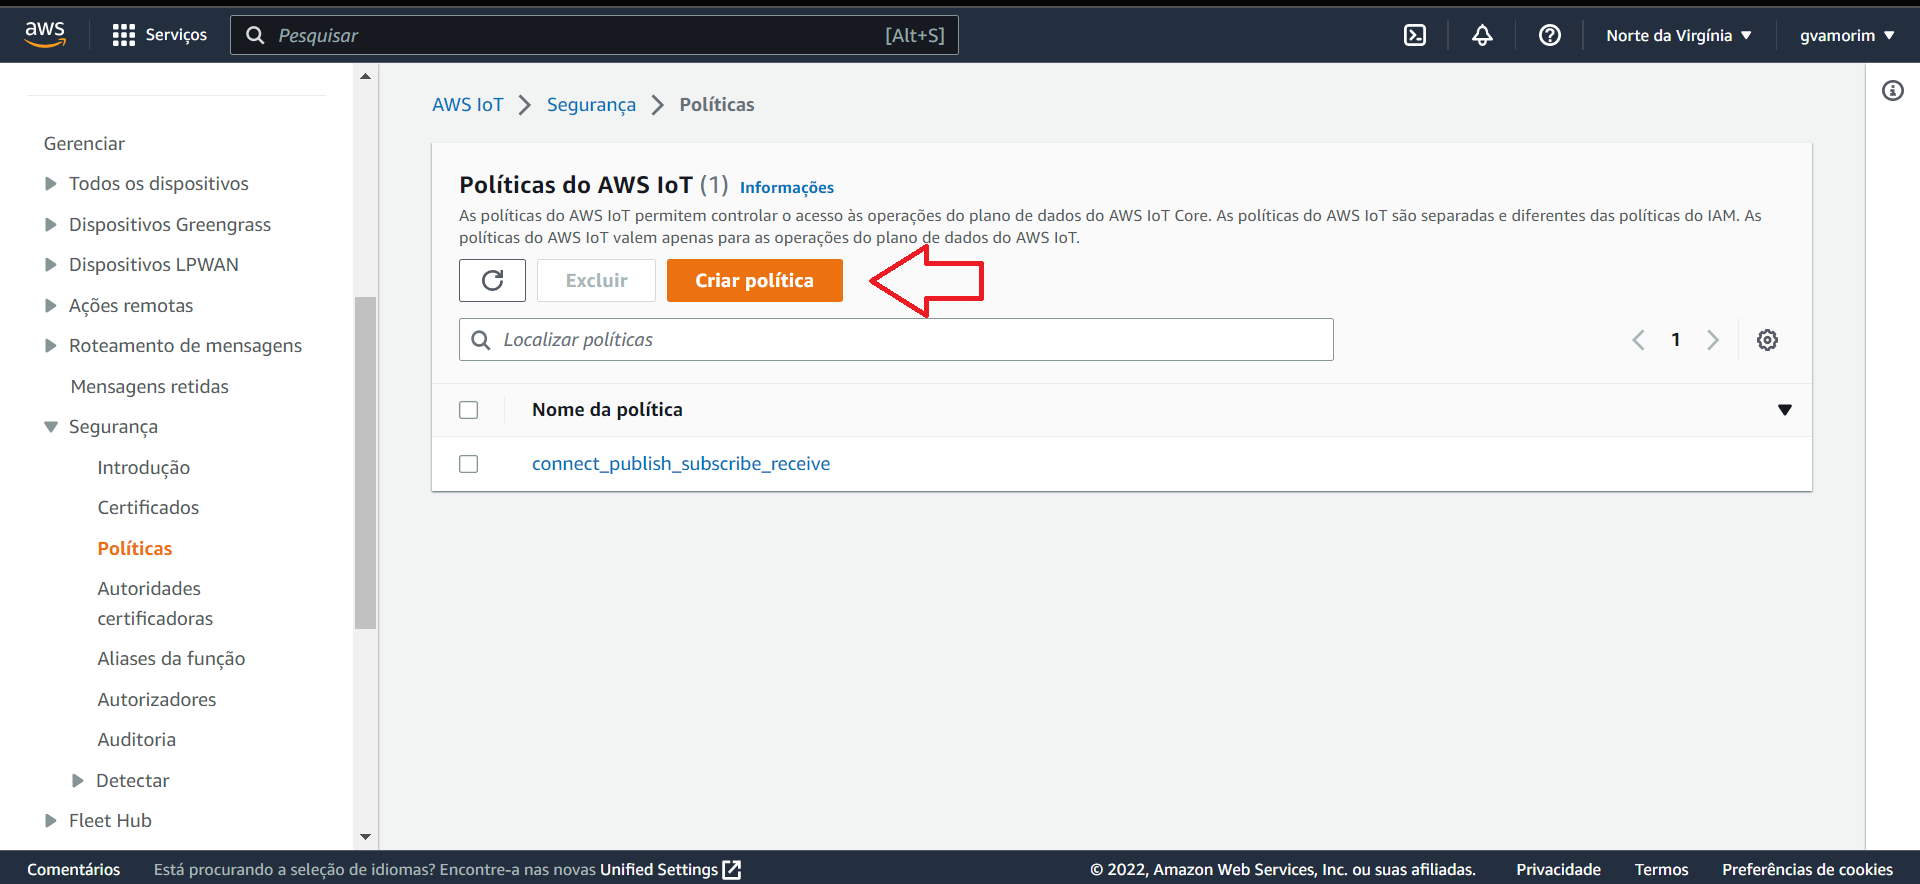
\includegraphics[scale=0.472]{Imagens/criando_uma_politica_no_aws_iot_1.png}
    \legend{Fonte: Produzido pelo autor (2022).}
    \label{fig:criando_uma_politica_no_aws_iot_b}
\end{figure}

Adicione um nome na opção \textit{Nome da política}.

\begin{figure}[H]
    \centering
    \caption{Criando uma política no AWS IoT (C).}
    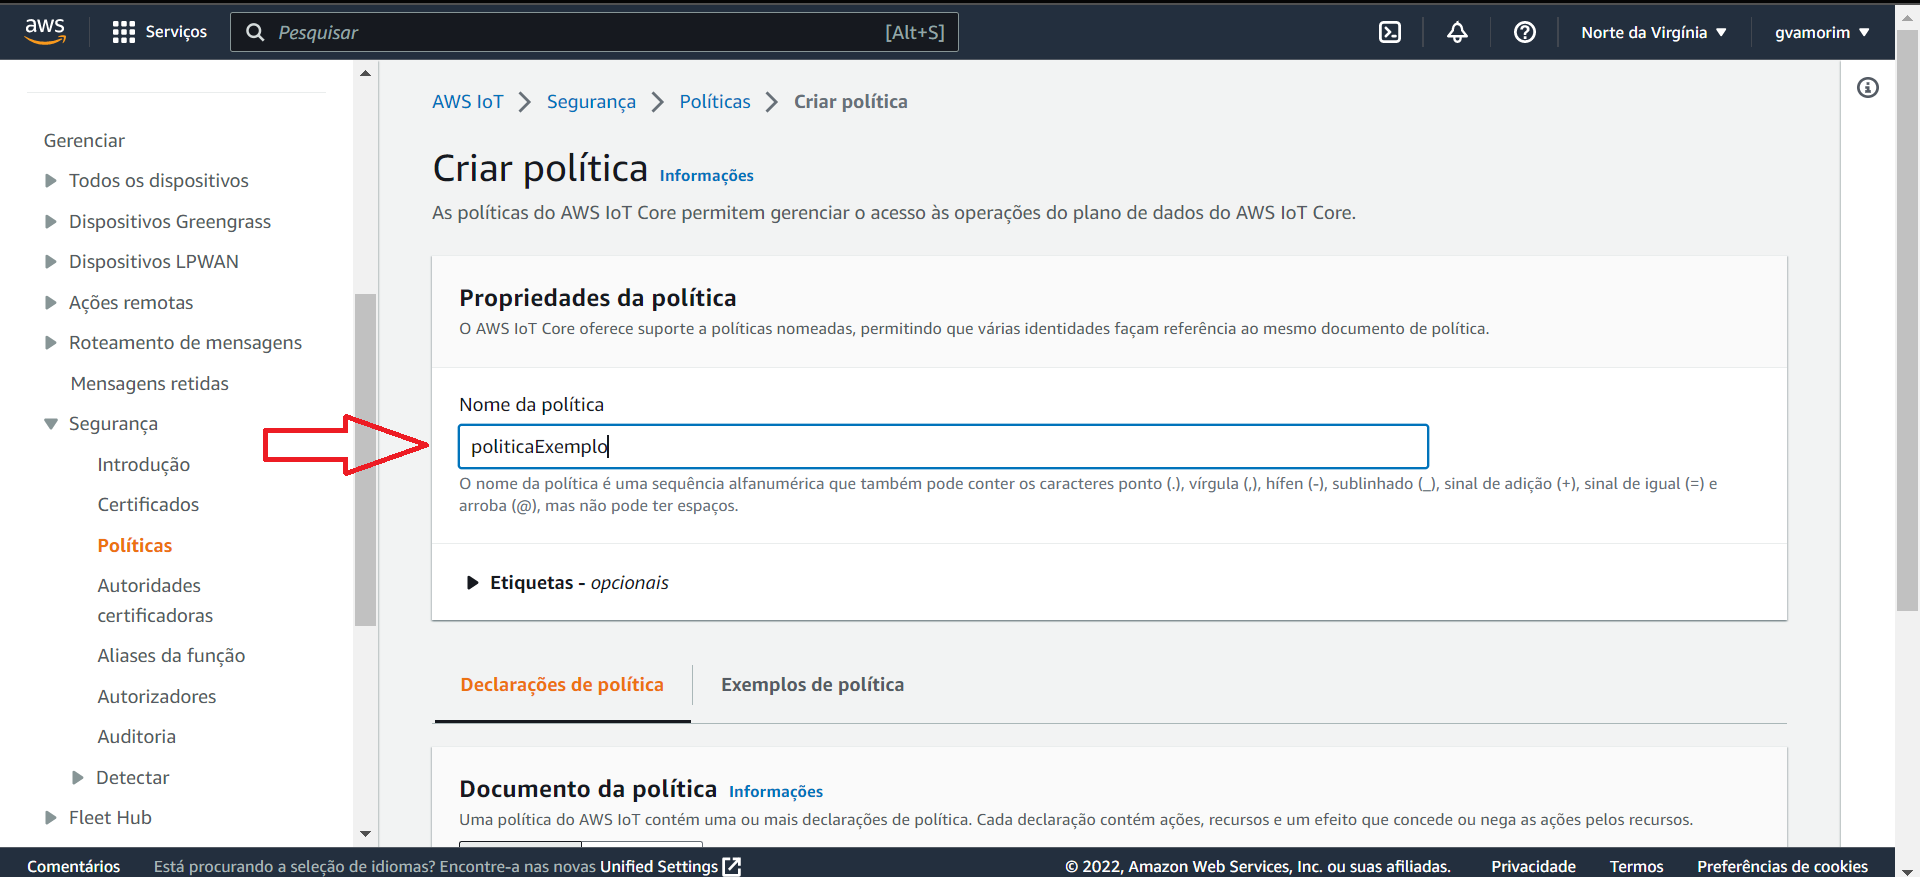
\includegraphics[scale=0.472]{Imagens/criando_uma_politica_no_aws_iot_2.png}
    \legend{Fonte: Produzido pelo autor (2022).}
    \label{fig:criando_uma_politica_no_aws_iot_c}
\end{figure}

Adicione declarações à política. As declarações podem ser adicionadas iterativamente (\autoref{fig:criando_uma_politica_no_aws_iot_d}) ou via documento JSON (\autoref{fig:criando_uma_politica_no_aws_iot_e}). O documento JSON da política utilizada no projeto foi apresentado no \autoref{lst:bl475e_policy}. Note que a opção \textit{Resource}, para cada declaração, segue o seguinte formato: ``arn:aws:iot: \textless regiao\textgreater:\textless id\_do\_usuario\textgreater:*''.

\begin{figure}[H]
    \centering
    \caption{Criando uma política no AWS IoT (D).}
    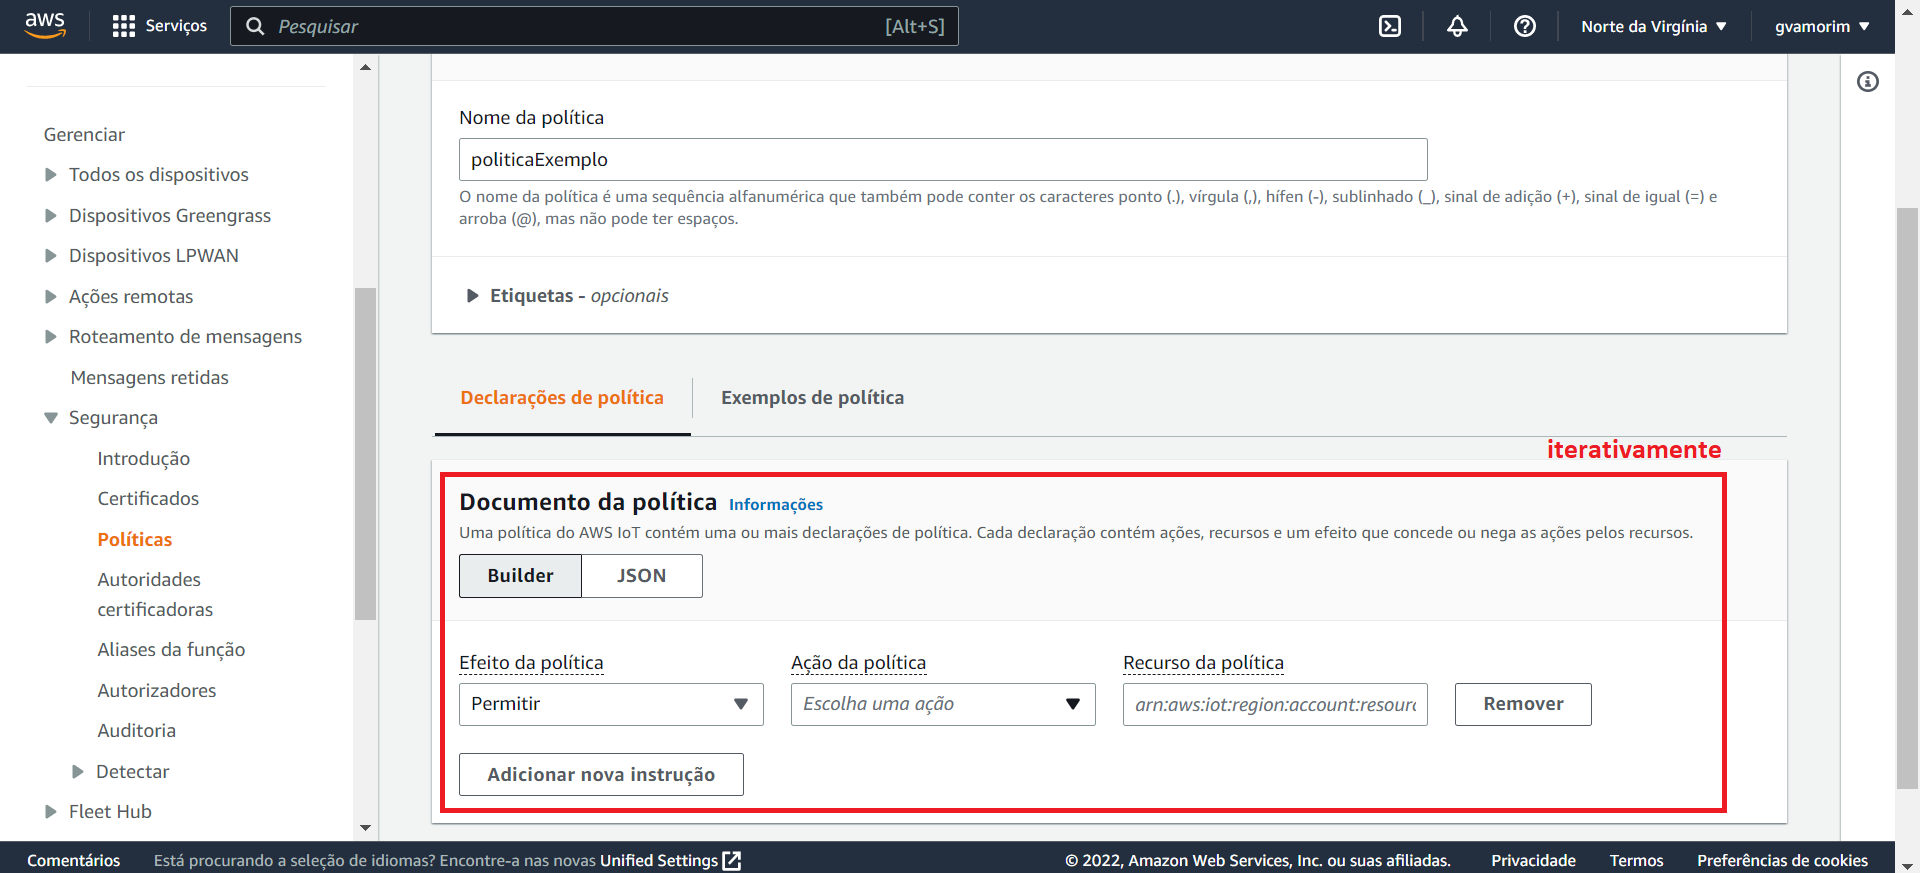
\includegraphics[scale=0.472]{Imagens/criando_uma_politica_no_aws_iot_3.png}
    \legend{Fonte: Produzido pelo autor (2022).}
    \label{fig:criando_uma_politica_no_aws_iot_d}
\end{figure}

\begin{figure}[H]
    \centering
    \caption{Criando uma política no AWS IoT (E).}
    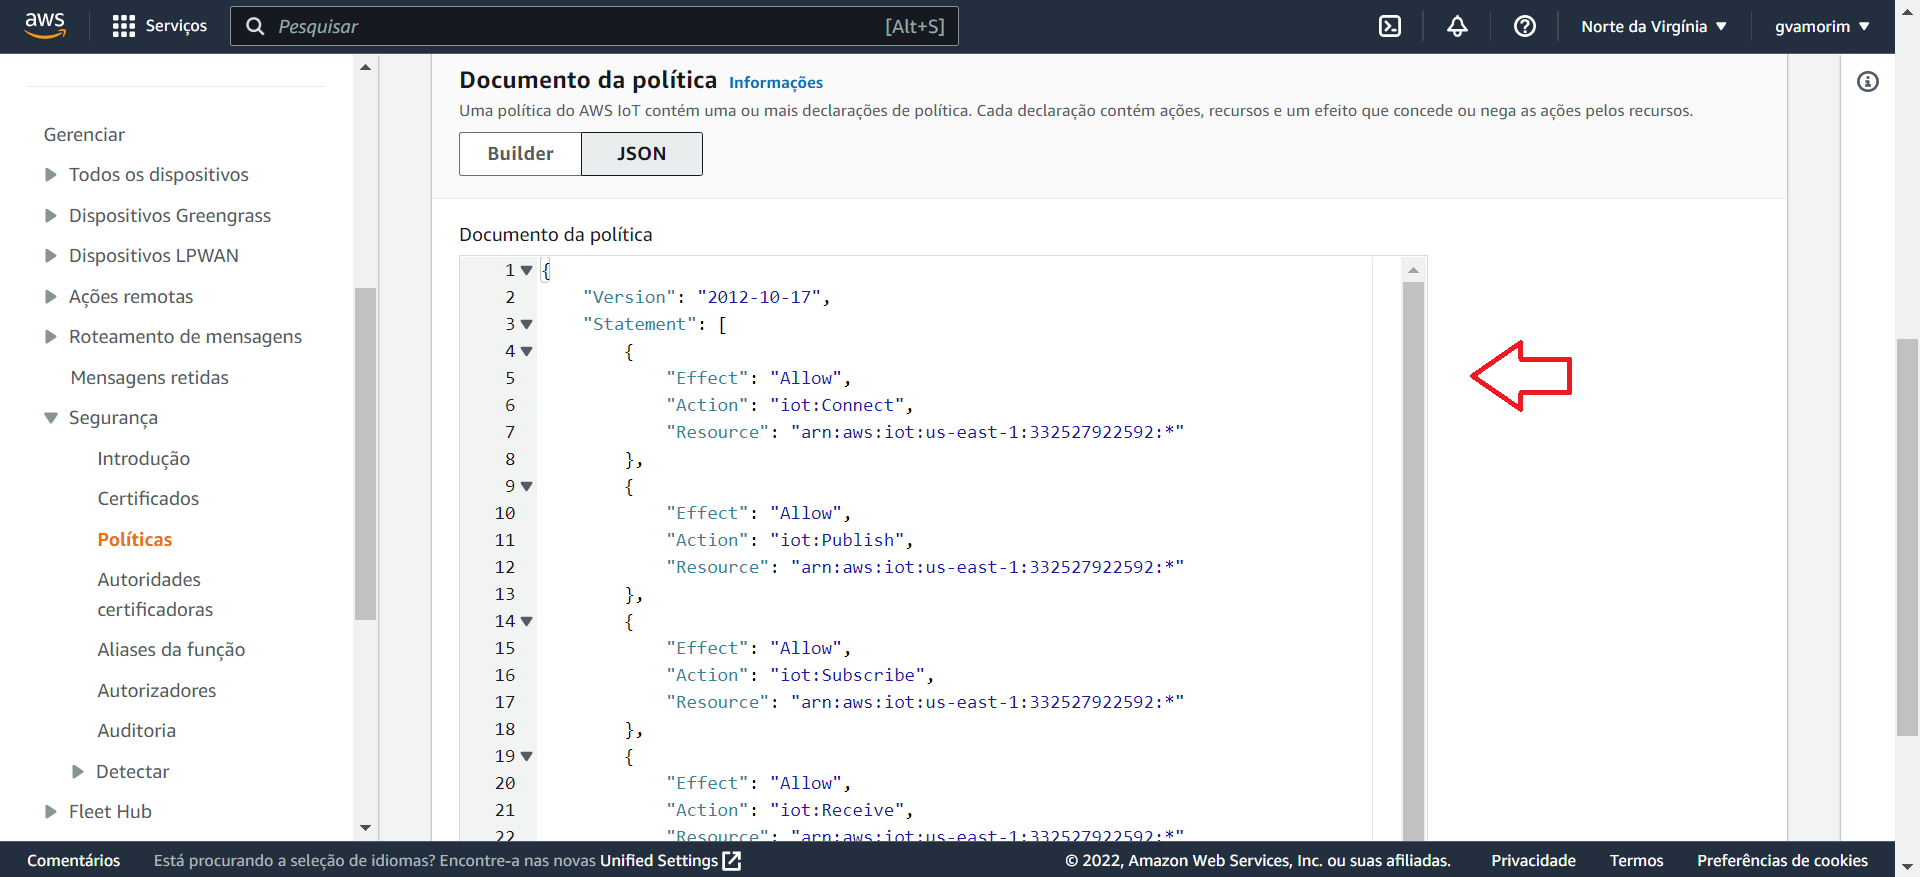
\includegraphics[scale=0.472]{Imagens/criando_uma_politica_no_aws_iot_4.png}
    \legend{Fonte: Produzido pelo autor (2022).}
    \label{fig:criando_uma_politica_no_aws_iot_e}
\end{figure}

Selecione a opção \textit{Criar}.

\begin{figure}[H]
    \centering
    \caption{Criando uma política no AWS IoT (F).}
    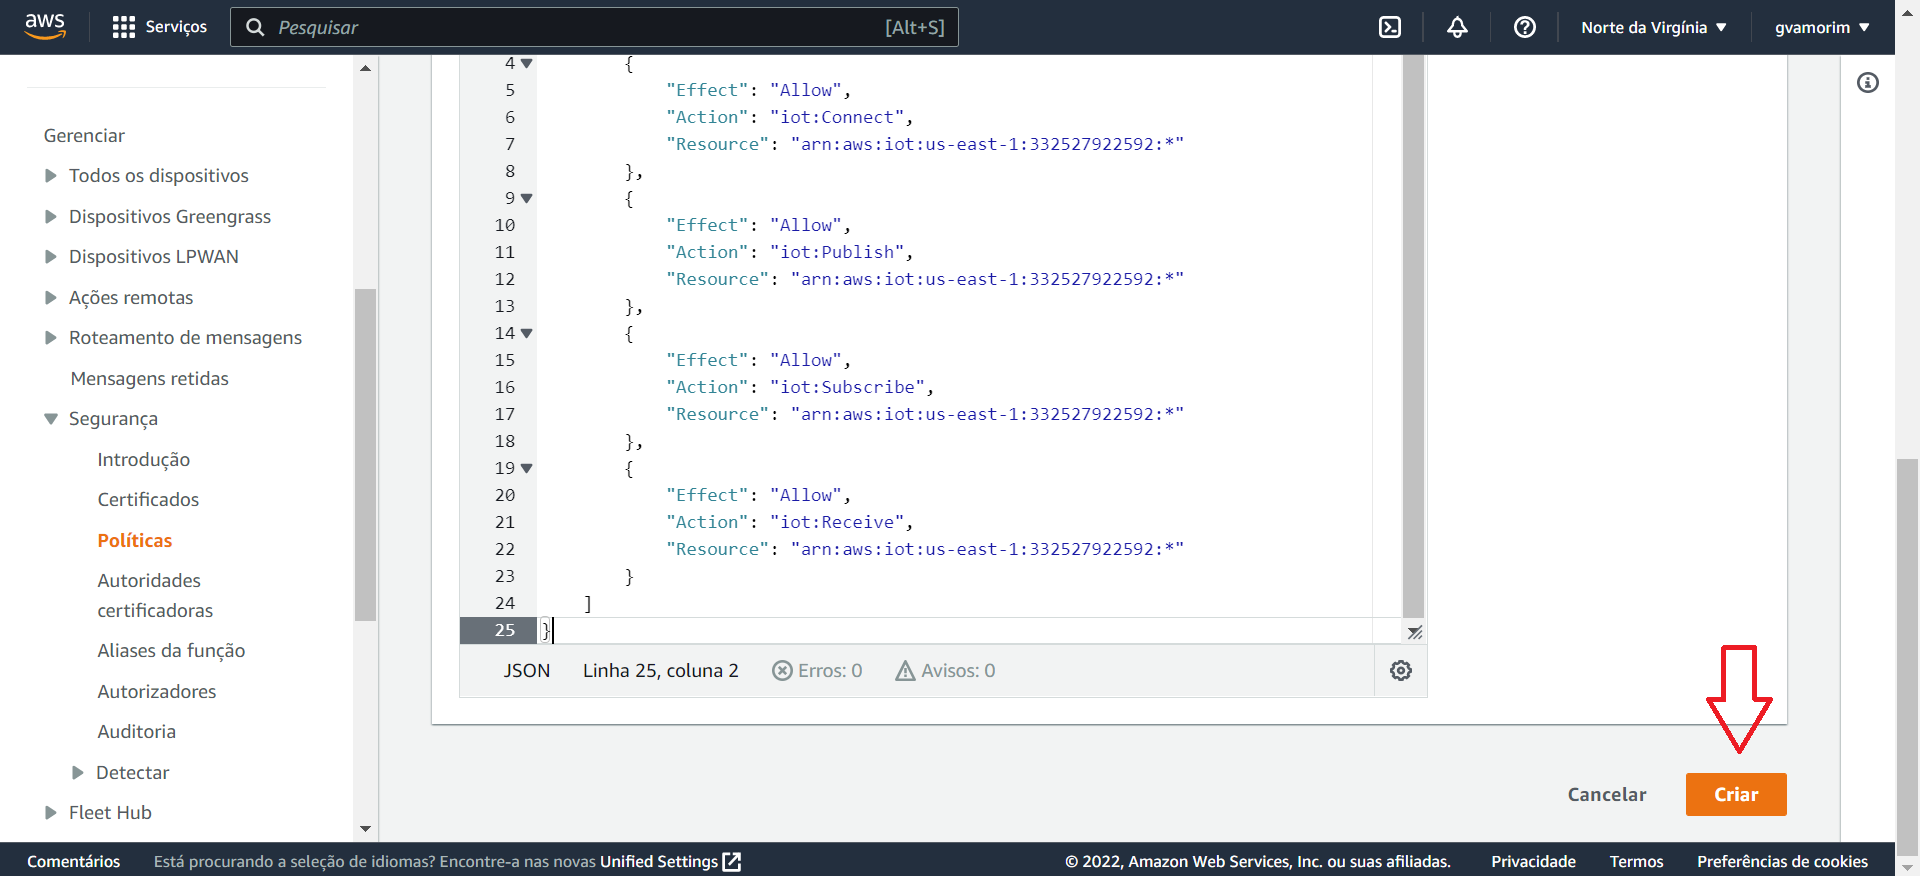
\includegraphics[scale=0.472]{Imagens/criando_uma_politica_no_aws_iot_5.png}
    \legend{Fonte: Produzido pelo autor (2022).}
    \label{fig:criando_uma_politica_no_aws_iot_f}
\end{figure}


% -----------------------------------------------------------------------------
% Capítulo A.2 - Criação de uma coisa no AWS IoT
% -----------------------------------------------------------------------------
\section{Criação de uma coisa no AWS IoT}\label{section:criacao_de_uma_coisa_no_aws_iot}

A sequência de figuras \autoref{fig:criacao_de_uma_coisa_no_aws_iot_a} até \autoref{fig:criacao_de_uma_coisa_no_aws_iot_g} apresentam capturas de telas do processo de criação de uma coisa no AWS IoT.

Acesse a \href{https://us-east-1.console.aws.amazon.com/iot/home?region=us-east-1#/home}{página principal do serviço AWS IoT}, expanda a opção \textit{Todos os Dispositivos} e selecione \textit{coisas}.

\begin{figure}[H]
    \centering
    \caption{Criando uma coisa no AWS IoT (A).}
    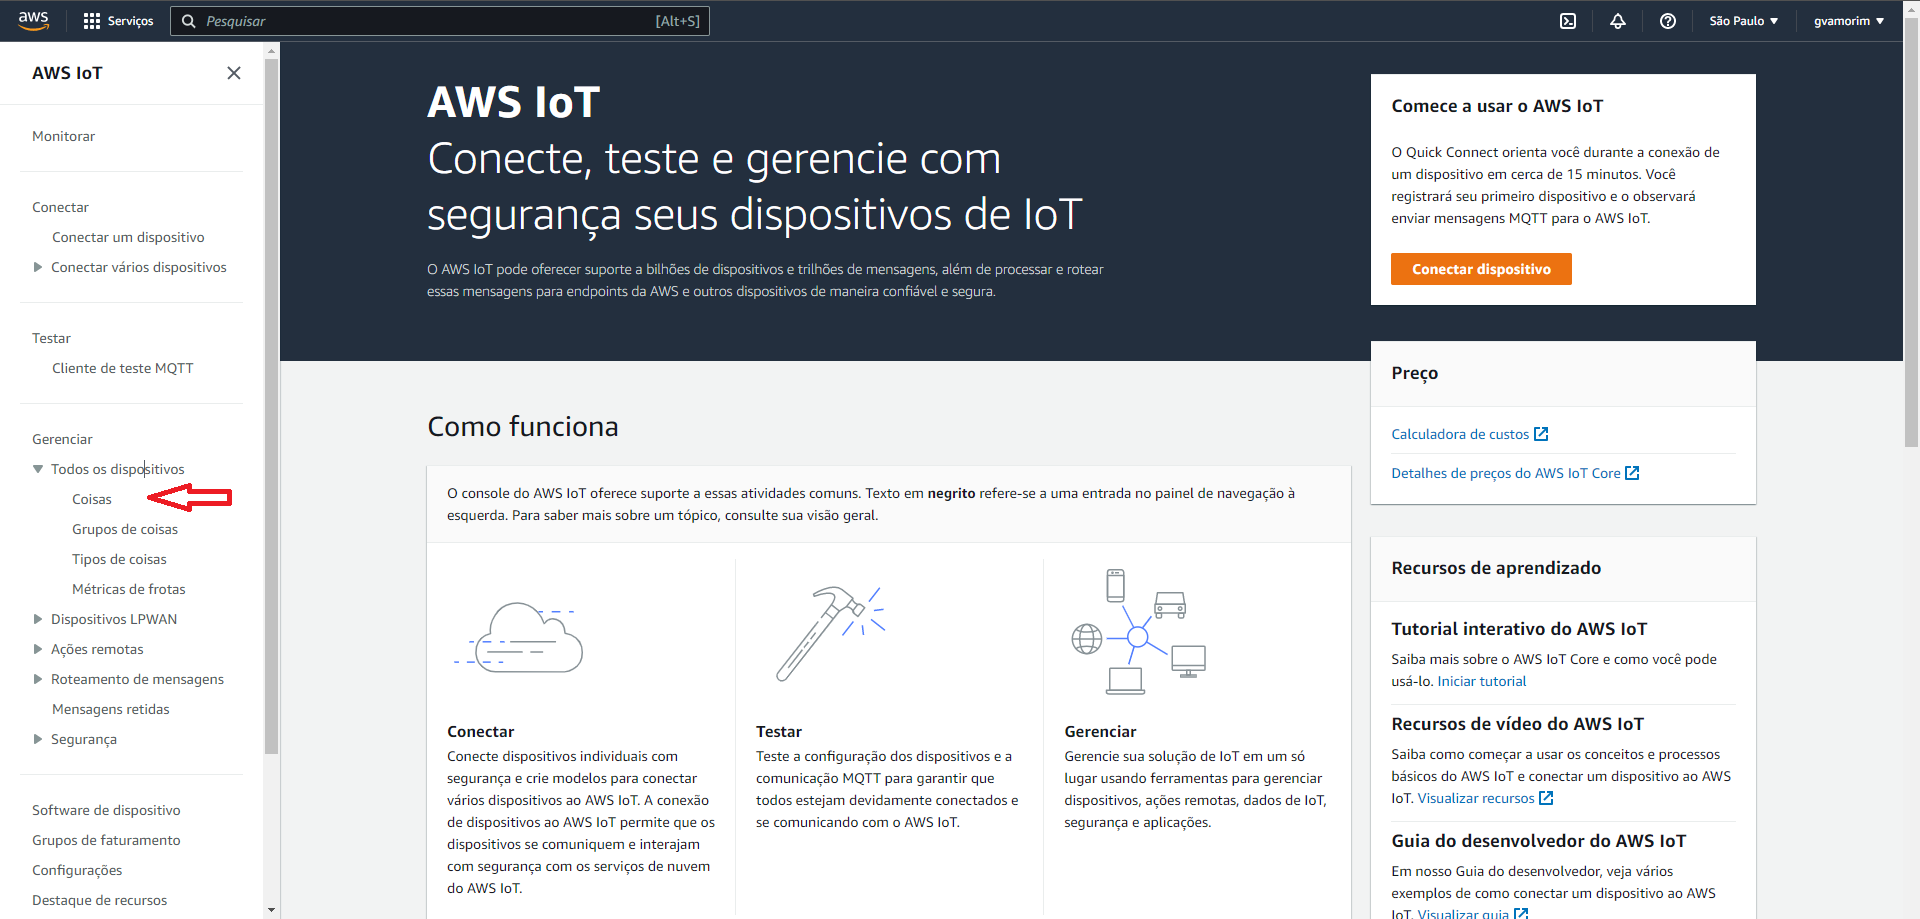
\includegraphics[scale=0.315]{Imagens/criando_uma_coisa_no_aws_iot_0.png}
    \legend{Fonte: Produzido pelo autor (2022).}
    \label{fig:criacao_de_uma_coisa_no_aws_iot_a}
\end{figure}

Selecione a opção \textit{Criar items}.

\begin{figure}[H]
    \centering
    \caption{Criando uma coisa no AWS IoT (B).}
    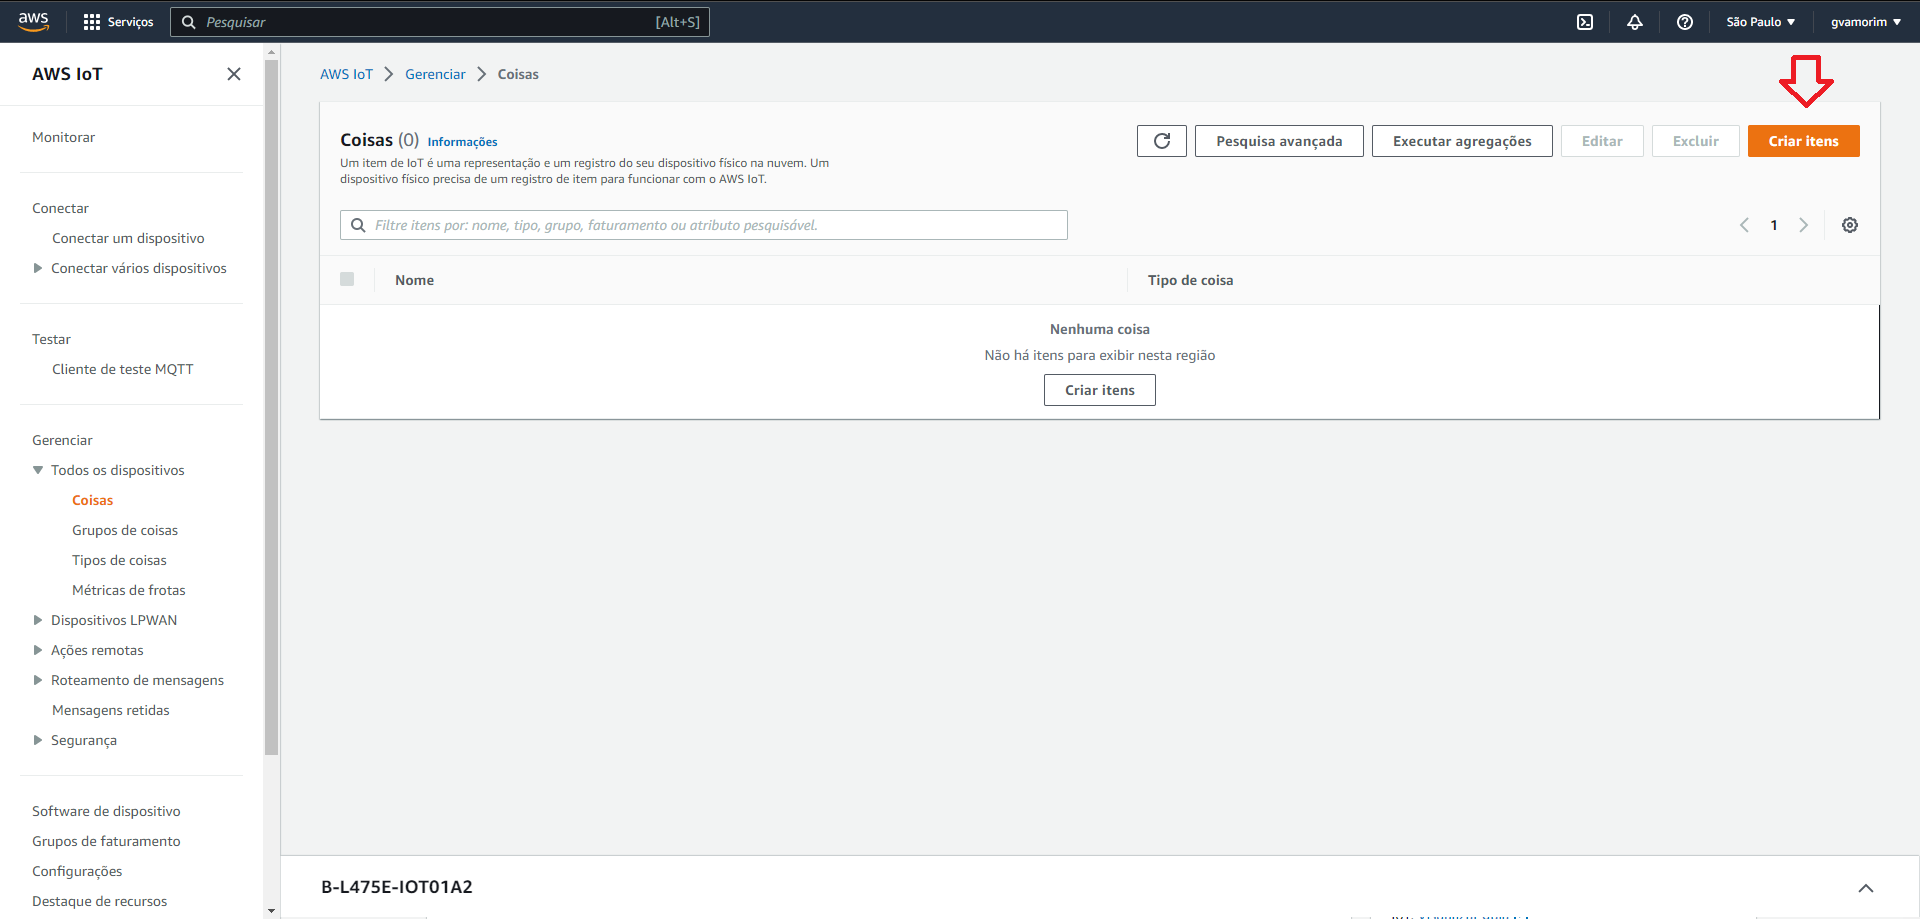
\includegraphics[scale=0.315]{Imagens/criando_uma_coisa_no_aws_iot_1.png}
    \legend{Fonte: Produzido pelo autor (2022).}
\end{figure}

Selecione a opção \textit{Criar um único item}.

\begin{figure}[H]
    \centering
    \caption{Criando uma coisa no AWS IoT (C).}
    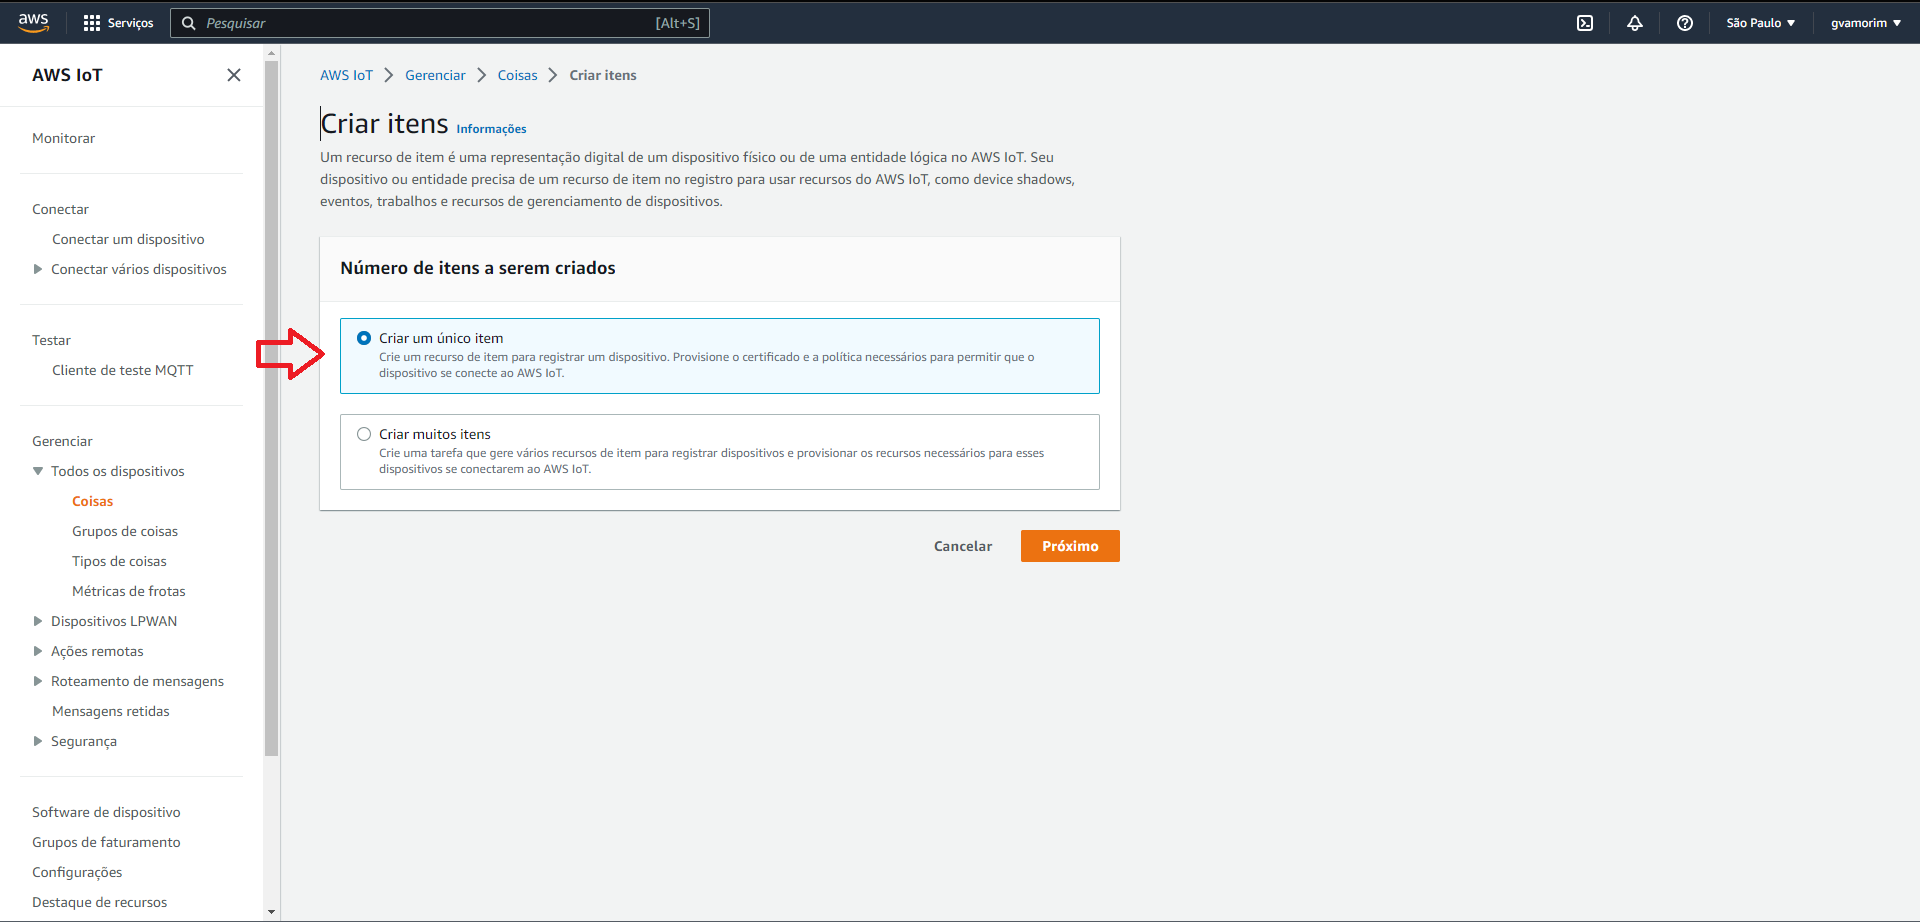
\includegraphics[scale=0.315]{Imagens/criando_uma_coisa_no_aws_iot_2.png}
    \legend{Fonte: Produzido pelo autor (2022).}
\end{figure}

Adicione um nome na opção \textit{Nome da coisa} e selecione \textit{Sombra sem nome (clássico)}.

\begin{figure}[H]
    \centering
    \caption{Criando uma coisa no AWS IoT (D).}
    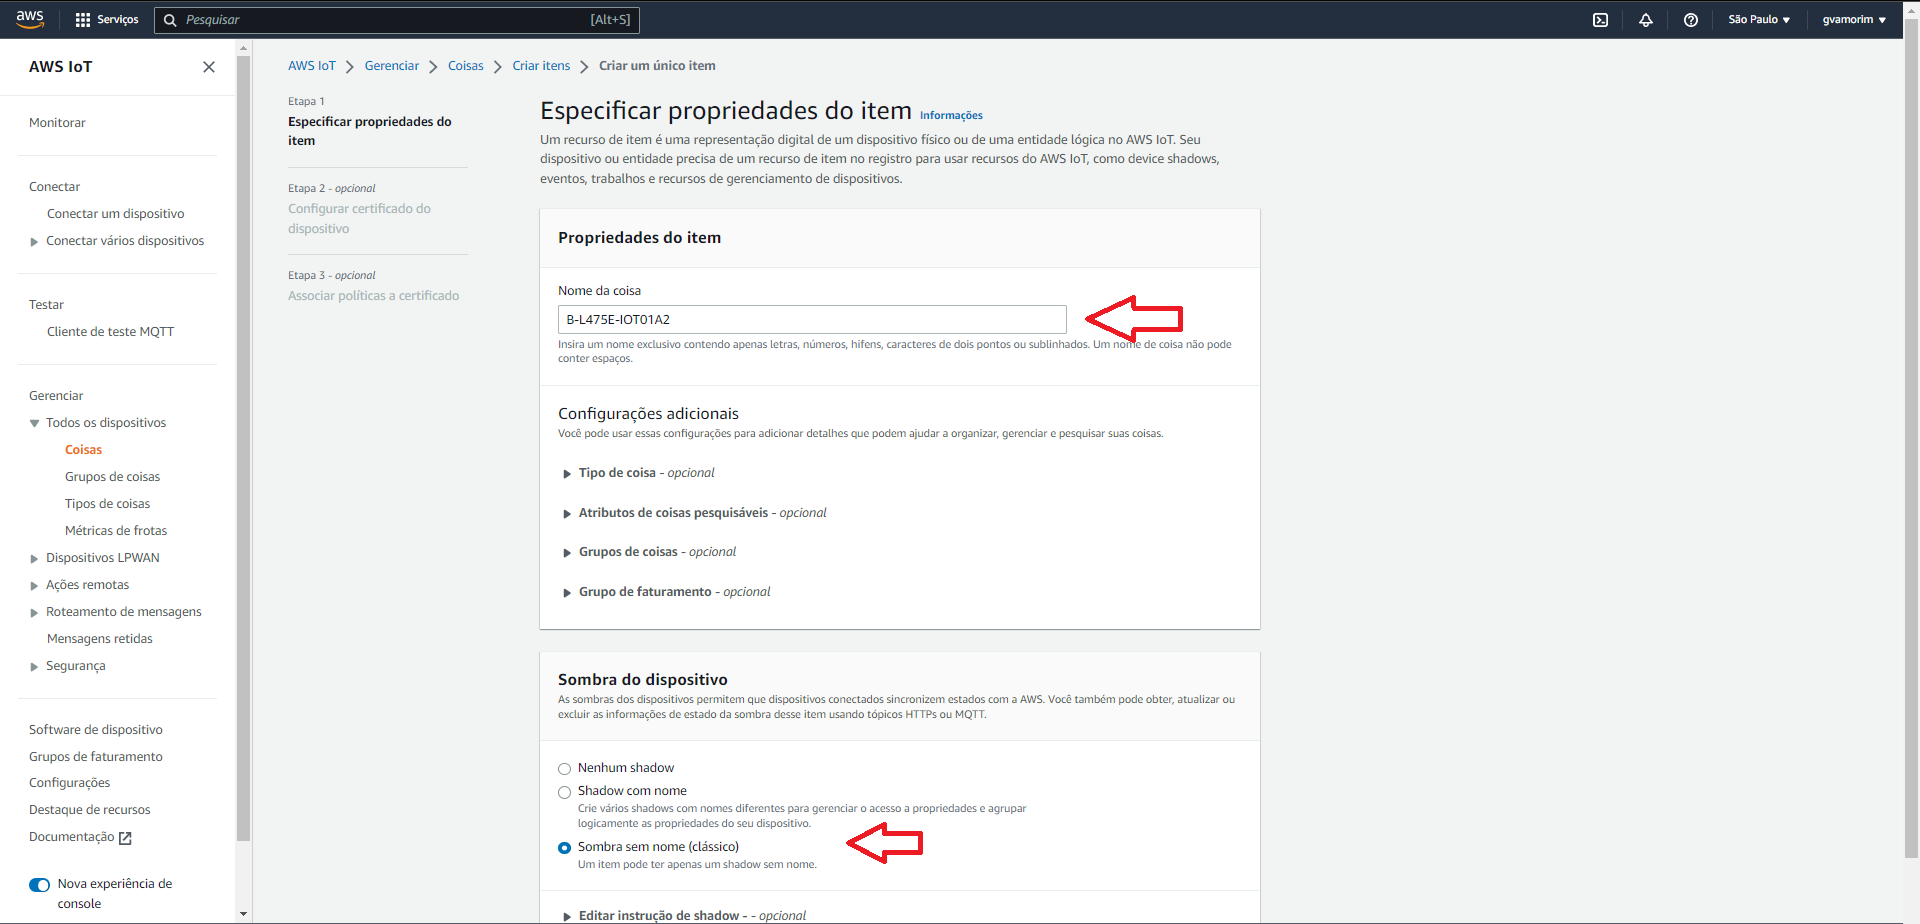
\includegraphics[scale=0.315]{Imagens/criando_uma_coisa_no_aws_iot_3.png}
    \legend{Fonte: Produzido pelo autor (2022).}
\end{figure}

Selecione a opção \textit{Gerar um novo certificado automaticamente (recomendado)}. Um dispositivo requer um certificado para conectar-se ao AWS IoT.

\begin{figure}[H]
    \centering
    \caption{Criando uma coisa no AWS IoT (E).}
    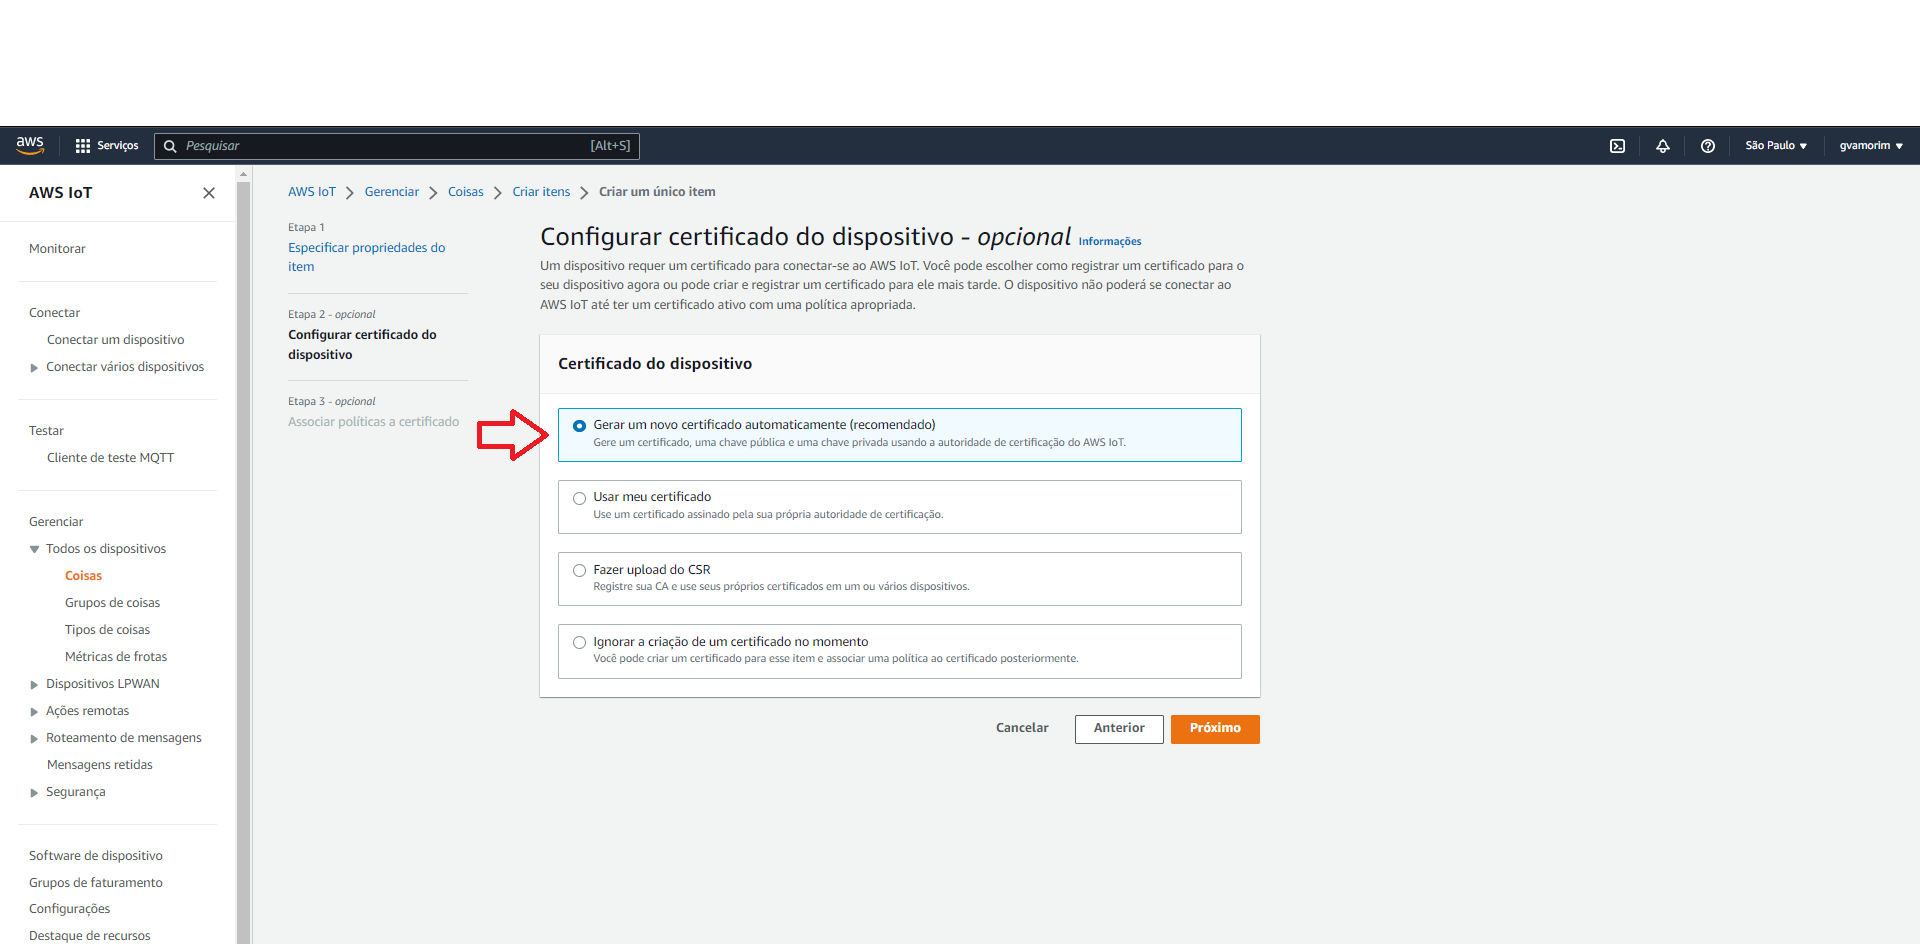
\includegraphics[scale=0.315]{Imagens/criando_uma_coisa_no_aws_iot_4.png}
    \legend{Fonte: Produzido pelo autor (2022).}
\end{figure}

Adicione uma política ao certificado. As políticas do AWS IoT concedem ou negam acesso a recursos do AWS IoT. O processo de criação de uma política para o AWS IoT foi descrito na \autoref{section:criacao_de_uma_politica_para_o_aws_iot}.

\begin{figure}[H]
    \centering
    \caption{Criando uma coisa no AWS IoT (F).}
    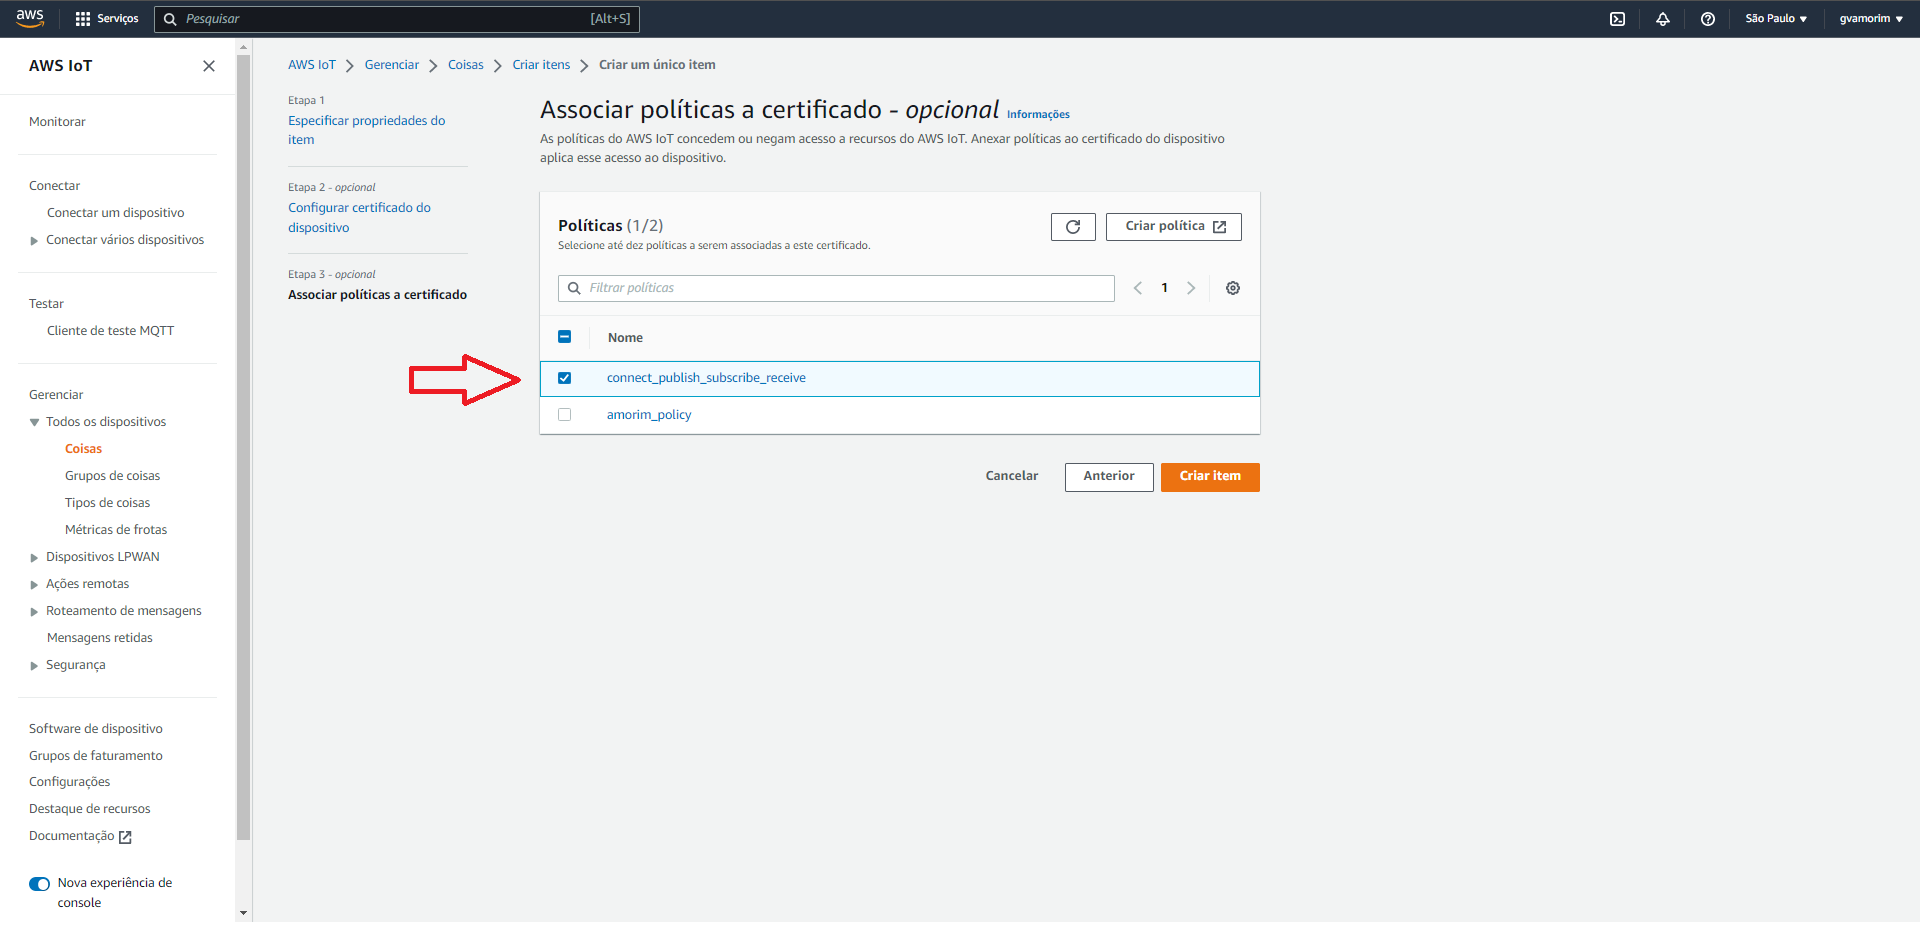
\includegraphics[scale=0.315]{Imagens/criando_uma_coisa_no_aws_iot_5.png}
    \legend{Fonte: Produzido pelo autor (2022).}
\end{figure}

Por fim, a coisa já está pronta no serviço AWS. Faça o \textit{download} dos certificados para que sejam instalados no dispositivo para que este possa se conectar à AWS.

\begin{figure}[H]
    \centering
    \caption{Criando uma coisa no AWS IoT (G).}
    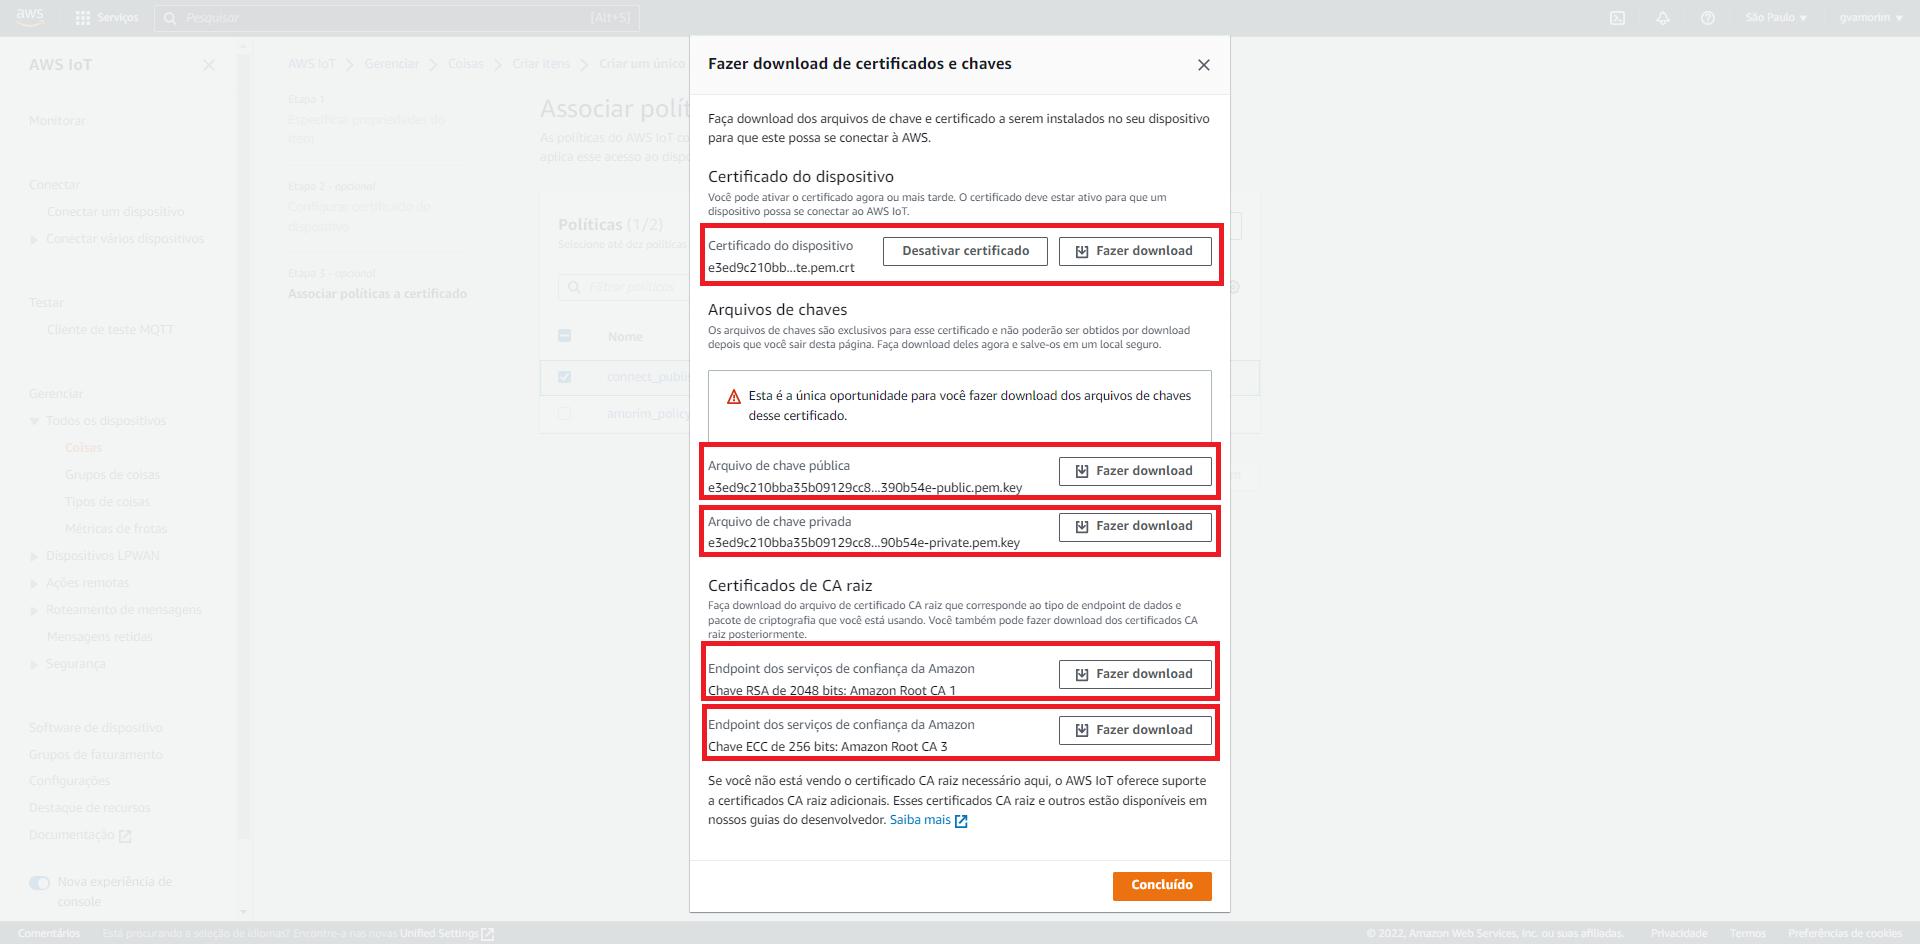
\includegraphics[scale=0.315]{Imagens/criando_uma_coisa_no_aws_iot_6.png}
    \legend{Fonte: Produzido pelo autor (2022).}
    \label{fig:criacao_de_uma_coisa_no_aws_iot_g}
\end{figure}

\section{Configuração do dispositivo B-L475E-IOT01A2 via USB usando o aplicativo Tera Term}\label{section:configuracao_dispositivo_bl475eiot01a2_via_usb}

A configuração do dispositivo B-L475E-IOT01A2 foi feita seguindo o tutorial da STMicroelectronics \cite{ref:041}.
